\chapter{Exploring Rigidity \& Circle Packings}  % Is it Rigid?

\begin{flushleft}
So far, we have seen the various definitions of rigidity that we can use to identify whether a given framework is rigid. However, we have no methods or techniques we can use in order to \textit{test} for the rigidity of a framework. We also don't know how the various definitions of rigidity get along with each other. If a framework is rigid, does it mean its infinitesimally rigid? Can we test for infinitesimal rigidity in some way? % find a third question
\end{flushleft}

\begin{flushleft}
In addition to these questions, we will also introduce circle packings, and discuss how they come about. As rigidity can't be tested merely by observation, testing the rigidity of a circle packing arises from using a few techniques seen earlier. For the remainder of this project, we will be working exclusively in $\mathbb{R}^2$ unless specified otherwise.
\end{flushleft}

\section{Degrees of Freedom}

\noindent
This section has been adapted from Graver's book \cite{counting_frameworks}.

\begin{flushleft}
To understand what it means for a framework to have $x$ number of \textit{degrees of freedom}, let us first go through some simple examples to gain an understanding of what a degree of freedom is.

\begin{itemize}
    \item Consider a point in $\mathbb{R}^2$. It can move right or left along the $x$-axis, or up and down along the $y$-axis. As it can travel along either axis, we say that this point has two \textit{degrees of freedom}. 
    \item Now, if we consider a line segment $l$ in the plane with two endpoints, we know that each endpoint has two degrees of freedom, giving us four degrees of freedom, but the line between them prevents the endpoints from moving independently of each other. So, $l$ can move either along the $x$ or $y$-axes, giving us two degrees of freedom. However, it can also rotate about some point in $\mathbb{R}^2$. Therefore, such a segment has three degrees of freedom.
    \item If we were to consider a point in $\mathbb{R}^3$, then as the point can travel along the $x$, $y$ or $z$-axes, it has three degrees of freedom. 
\end{itemize}
\end{flushleft}

\begin{flushleft}
At this point, we should be able to see what a degree of freedom means. It is essentially a count of how many ways we can move a structure (or frameworks in our case) around in space. Additionally, we can note that adding an edge between two points reduces the total degrees of freedom in the system from four to three due to the constraint that the points can't move independently of each other. 
\end{flushleft}
\vspace{-3 mm}
\begin{figure}[htbp]
    \centering
    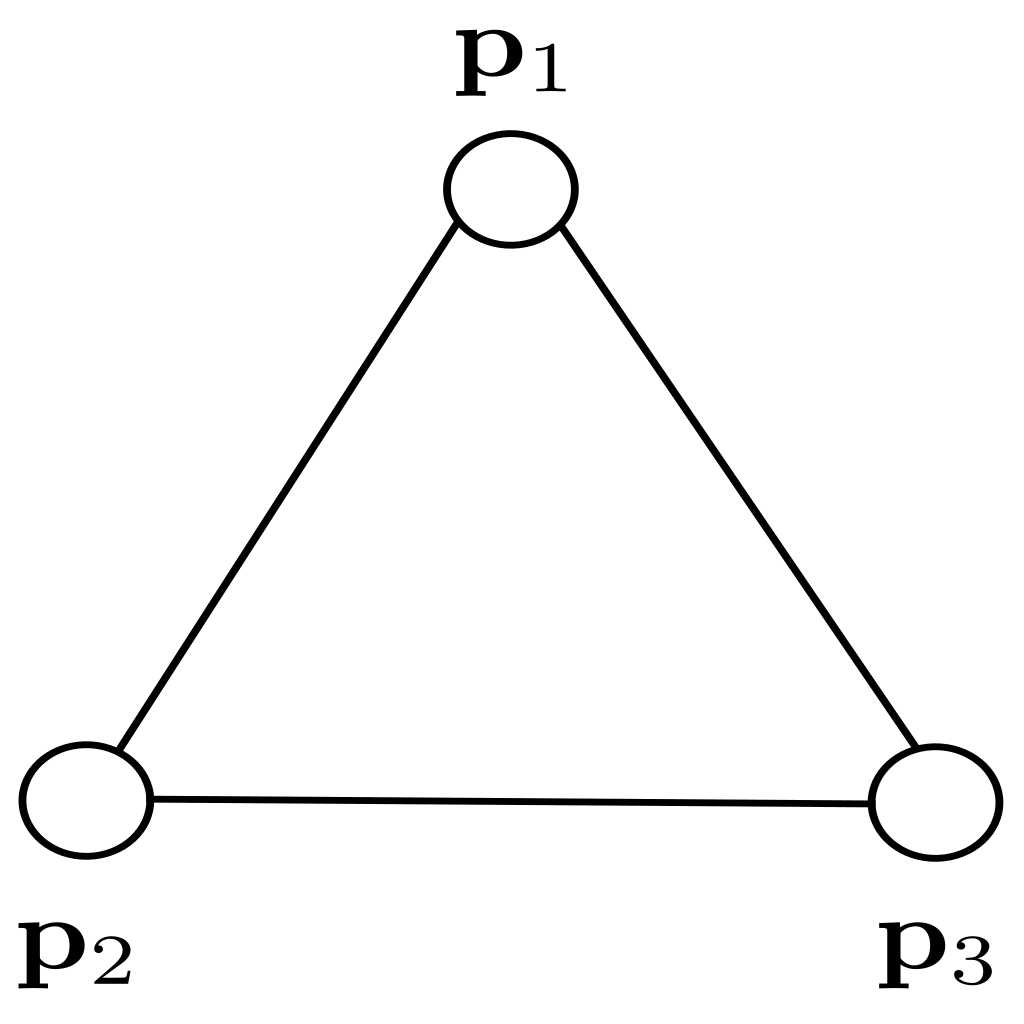
\includegraphics[width = 0.25\textwidth]{Chapter 3/5. degree_of_freedom.png}
    \caption{A framework on three nodes and three edges}
    \label{fig: degree_of_freedom}
\end{figure}

\begin{example}
In order to find how many degrees of freedom the framework in Figure \ref{fig: degree_of_freedom} has, we start with just three nodes, and then build up to the framework given:
\begin{itemize}
    \item With only three nodes in the plane, and each node having two degrees of freedom, the total degrees of freedom the system has is $3 \times 2 = 6$.
    \item If we add an edge between $\mathbf{p}_1$ and $\mathbf{p}_2$ now, we lose a degree of freedom, giving us $3$ degrees of freedom for the segment and $2$ for the segment, totalling $5$ degrees of freedom in the system.
    \item Adding the edge between $\mathbf{p}_1$ and $\mathbf{p}_3$, we further reduce the number of ways the framework can move: $3$ degrees of freedom for the first segment and $1$ degree of freedom for rotation of the second segment about their common endpoint. At this stage, the structure has $4$ degrees of freedom.
    \item Adding the last edge between $\mathbf{p}_2$ and $\mathbf{p}_3$ gives us the framework in question. We reduce the degrees of freedom by one yet again, giving us $3$ degrees of freedom in total now.
\end{itemize}
\end{example}

\begin{flushleft}
Using Definition \ref{def: rigid}, we know that for any (infinitesimally) rigid body in the plane, we must only be allowed to translate it along the two axes, as well as only rotate it about some point.
\end{flushleft}

\begin{theorem}
\label{thm: degrees of rigid body}
In $\mathbb{R}^2$, any rigid body must have $3$ degrees of freedom. 
\end{theorem}

\section{The Rigidity Matrix}

\begin{flushleft}
When given a framework, it can be quite difficult to tell whether it is rigid or not. This is where the \textit{rigidity matrix} comes in. By finding a way to encode a framework into a matrix, we can then use tools from linear algebra to study and draw conclusions about the framework itself!
\end{flushleft}

\begin{definition}
\label{def: rigidity matrix}
The \textit{rigidity matrix} $\mathbf{R}(G,\mathbf{p})$ of a $d$-dimensional framework $(G,\mathbf{p})$ is a matrix that contains the system of equations described in Definition \ref{def: inf motion}. It is a $|E(G)| \times d|V(G)|$ matrix, where the rows are indexed by the edges of $G$, and sets of $d$ consecutive columns correspond to a single node of $(G,\mathbf{p})$. 

\noindent
If there is an edge between nodes $\mathbf{p}_i$ and $\mathbf{p}_j$ when $d=2$, then the non-zero entries in the corresponding row of the matrix lie in columns corresponding to coordinates of each node. That is;
\begin{itemize}
    \item Columns $2i-1$ and $2i$ corresponding to the coordinates of node $p_i$.
    \item Columns $2j-1$ and $2j$ corresponding to the coordinates of node $p_j$.
    \item $0$ everywhere else.
\end{itemize}
\end{definition}

\begin{figure}[htbp]
    \centering
    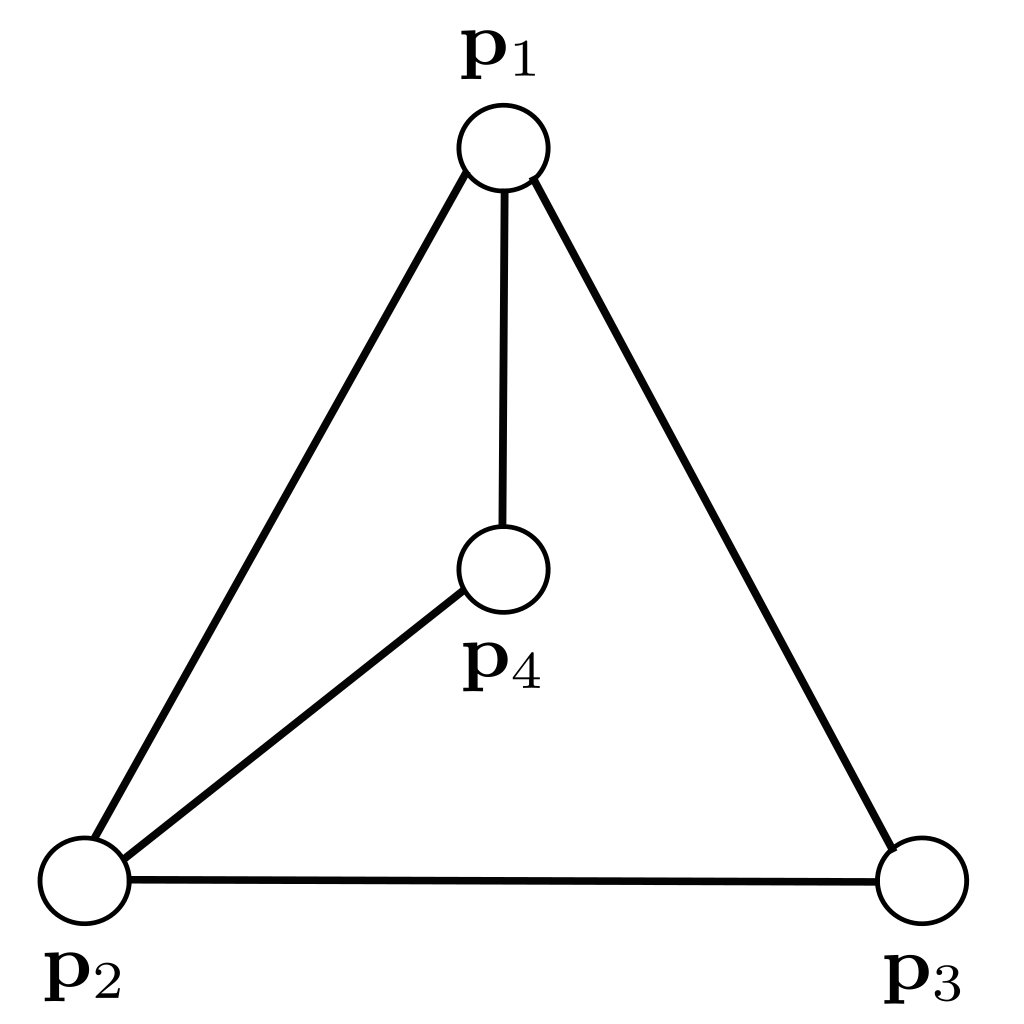
\includegraphics[width = 0.25\textwidth]{Chapter 3/4. rigidity_matrix.png}
    \caption{A framework on four nodes and five edges.}
    \label{fig: rigidity_matrix}
\end{figure}
\vspace{-3 mm}
\begin{flushleft}
For example, consider the framework $(G,\mathbf{p})$ in Figure \ref{fig: rigidity_matrix}. 
\end{flushleft}
%\vspace{20 mm} % allows for the text to flow smoother
\begin{flushleft}
As we are working in $\mathbb{R}^2$, we know that $\mathbf{p}_i = (x_{i}, y_{i})$, for each $i = 1,2,3,4$. Therefore, we can construct $\mathbf{R}(G,\mathbf{p})$ as
\end{flushleft}
\vspace{-6 mm}
\begin{center}
\begin{tabular}{ c c } 
 & \underline{Edges} \\
\multirow{5}{15 cm}{$
    \mathbf{R}(G,\mathbf{p}) = 
    \begin{bmatrix}
    x_1 - x_2 & y_1 - y_2 & x_2 - x_1 & y_2 - y_1 & 0 & 0 & 0 & 0 \\ %p1p2
    x_1 - x_3 & y_1 - y_3 & 0 & 0 & x_3 - x_1 & y_3 - y_1 & 0 & 0 \\ %p1p3
    x_1 - x_4 & y_1 - y_4 & 0 & 0 & 0 & 0 & x_4 - x_1 & y_4 - y_1 \\ %p1p4
    0 & 0 & x_2 - x_3 & y_2 - y_3 & x_3 - x_2 & y_3 - y_2 & 0 & 0 \\ %p2p3
    0 & 0 & x_2 - x_4 & y_2 - y_4 & 0 & 0 & x_4 - x_2 & y_4 - y_2 \\ %p2p4
    \end{bmatrix}$} & $\mathbf{p}_1\mathbf{p}_2$ \\
    & $\mathbf{p}_1\mathbf{p}_3$ \\
    & $\mathbf{p}_1\mathbf{p}_4$ \\
    & $\mathbf{p}_2\mathbf{p}_3$ \\
    & $\mathbf{p}_2\mathbf{p}_4$ \\    
\end{tabular}
\end{center}
\vspace{0.5 mm}
\begin{flushleft}
The rows of $\mathbf{R}(G,\mathbf{p})$ correspond to the edges in $(G,\mathbf{p})$, and each consecutive set of two columns correspond to the $x$ and $y$ coordinates of each node in $\mathbf{p}$, leading to the creation of $2 \times 4 = 8$ columns and $5$ rows in $\mathbf{R}(G,\mathbf{p})$.
\end{flushleft}

\begin{example}
\label{eg: rigidity matrix}
Let the framework $(G,\mathbf{p})$ be the one in Figure \ref{fig: rigidity_matrix}. If we give the nodes of $(G,\mathbf{p})$ positions in $\mathbb{R}^2$, we can compute its numeric rigidity matrix $\mathbf{R}(G,\mathbf{p})$. 

\noindent
Suppose that $\mathbf{p}_1 = (1,2)$, $\mathbf{p}_2 = (0,0)$, $\mathbf{p}_3 = (2,0)$, $\mathbf{p}_4 = (1,1)$. Then, the rigidity matrix $\mathbf{R}(G,\mathbf{p})$ is

\[
\mathbf{R}(G,\mathbf{p}) = 
\begin{bmatrix}
1 & 2 & -1 & -2 & 0 & 0 & 0 & 0 \\
-1 & 2 & 0 & 0 & 1 & -2 & 0 & 0 \\
0 & 1 & 0 & 0 & 0 & 0 & 0 & -1 \\
0 & 0 & -2 & 0 & 2 & 0 & 0 & 0 \\
0 & 0 & -1 & -1 & 0 & 0 & 1 & 1 \\
\end{bmatrix}
\]
\end{example}

\begin{flushleft}
Now that we have the rigidity matrix, we can use it to determine whether a given d-dimensional framework is infinitesimally rigid or not. Recalling Definition \ref{def: inf motion}, we can see that the space of infinitesimal motions of a framework $(G,\mathbf{p})$ is equal to the kernel of $R(G,\mathbf{p})$, denoted Ker($\mathbf{R}$).

By using a result from Linear Algebra known as the \textbf{Rank-Nullity Theorem}, we see that
\vspace{-1 mm}
\[
\text{rank}(\mathbf{R}) + \text{dim}(\text{Ker}(\mathbf{R})) = d|V|
\]

\end{flushleft}

\begin{flushleft}
As the space of infinitesimal rigid motions govern the number of ways a framework can move in space, we can deduce that a useful result.
\end{flushleft}

\begin{lemma}
Let $(G,\mathbf{p})$ be a framework, and $\mathbf{R}(G,\mathbf{p})$ be its rigidity matrix. Then $(G,\mathbf{p})$ has $dim(\text{Ker}(\mathbf{R}))$ degrees of freedom. 
\end{lemma}

\begin{flushleft}
As we're concerned with frameworks in $\mathbb{R}^2$, using Theorem \ref{thm: degrees of rigid body}, we know that rigid frameworks must have $3$ degrees of freedom. From Definition \ref{def: inf rigid}, we deduce the following theorem.
\end{flushleft}

\begin{theorem}
\label{thm: rank-rigid}
Let $(G,\mathbf{p})$ be a framework and $\mathbf{R}(G,\mathbf{p})$ be its rigidity matrix. Then, $(G,\mathbf{p})$ is infinitesimally rigid in $\mathbb{R}^2$ if and only if 
\[
\text{rank}(\mathbf{R}) = 2|V| - 3
\]
\end{theorem}

\begin{flushleft}
We have now successfully used techniques from linear algebra in order to test for infinitesimal rigidity of a framework! This result was proved by Asimow and Roth in their paper \cite{asimow}, and is going to be a pertinent to this project. Being able to analyze frameworks using matrices enables us to computationally investigate properties of the matrix, allowing for a speedy analysis of a given framework.
\end{flushleft}

\section{Constructing Rigid Structures}
Through an algorithmic process of adding nodes and deleting edges, we can create frameworks such that they are rigid in nature. This is done using the Henneberg construction \cite{henneberg}. However, in order to end up with a rigid framework, we must start with a graph known as a \textit{Laman Graph}.

\begin{definition}
\label{def: laman graph}
Let $G = (V,E)$ be a connected graph, and let $H$ be a subgraph of $G$. Then $G$ is known as a \textit{Laman graph} if
\begin{itemize}
    \item The edge set of $G$ has size $|E(G)| = 2|V(G)| - 3$.
    \item For any subgraph $H$ defined on $k \leq |V(G)|$ vertices, $|E(H)| \leq 2k-3$.
\end{itemize}
as defined in \cite{laman_graph}.
\end{definition}

\begin{flushleft}
Such graphs are named after Gerard Laman, who studied the rigidity of graphs in the 1970s. 

Now, a question we can ask at this stage is if we can find graphs that are rigid on the smallest number of edges possible. That is, are there rigid graphs such that if we take away an edge, it causes the structure to lose its rigidity? Such graphs are known to be \textit{minimally rigid}.
\end{flushleft}

\begin{flushleft}
As this project revolves around minimally rigid graphs, it is important to learn what graphs are minimally rigid, and if there's a way to identify which graphs are classed as minimally rigid. 
\end{flushleft}

\begin{theorem}
\label{thm: laman = minimally rigid}
A graph $G$ is minimally rigid in $\mathbb{R}^2$ if and only if $G$ is a Laman graph \cite{minimally_rigid}.
\end{theorem}

\begin{flushleft}
Therefore, a graph $G$ is minimally rigid if and only if $G$ has $2n-3$ edges, where $n = |V(G)|$. This is known as the Geiringer–Laman theorem, as it was first proved by Hilda Pollaczek-Geiringer in 1927 \cite{laman_theorem}, and then independently by Laman in 1970 \cite{minimally_rigid}.
\end{flushleft}

\begin{flushleft}
Given such a characterization, we can now talk about ways to construct minimally rigid graphs, of which there are two we focus on. They are known as the \textit{Henneberg constructions} \cite{henneberg}.
\end{flushleft}

\begin{definition}
\label{def: henneberg}
The \textit{Henneberg construction} in $\mathbb{R}^2$ involves two processes in order to generate minimally rigid graphs.
\begin{itemize}
    \item Type I: To an existing Laman graph $G$, insert a new vertex $u$ and attach it to $G$ by adding two edges between $u$ and two distinct vertices in $G$.
    \item Type II: To an existing Laman graph $G$, delete an edge between two vertices $v_1,v_2 \in V(G)$, insert a new vertex $u$, and attach it to $G$ by adding edges between $u$ and $v_1$, $v_2$ and one other vertex in $G$. 
\end{itemize}
\noindent
The resulting graph will be have $2|V(G)|-3$ edges, and is therefore minimally rigid by Theorem \ref{thm: laman = minimally rigid}.
\end{definition}

\begin{example}
A sequence of constructions using Henneberg Type I and Type II are shown.

\begin{figure}[htbp]
    \centering
    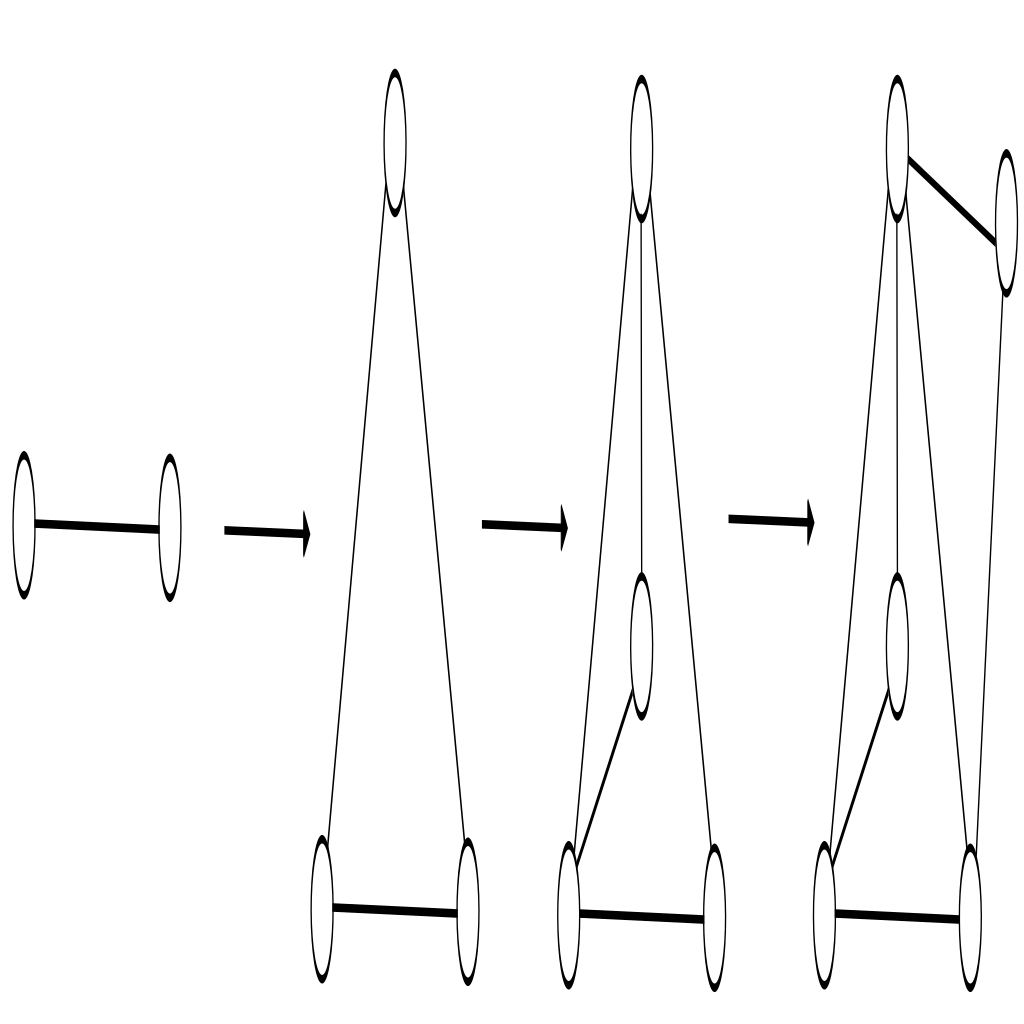
\includegraphics[width = 0.9\textwidth]{Chapter 3/2. henneberg_1.png}
    \caption{A series of constructions created solely using Henneberg Type I}
    \label{fig: henneberg 1}
\end{figure}

\begin{figure}[htbp]
    \centering
    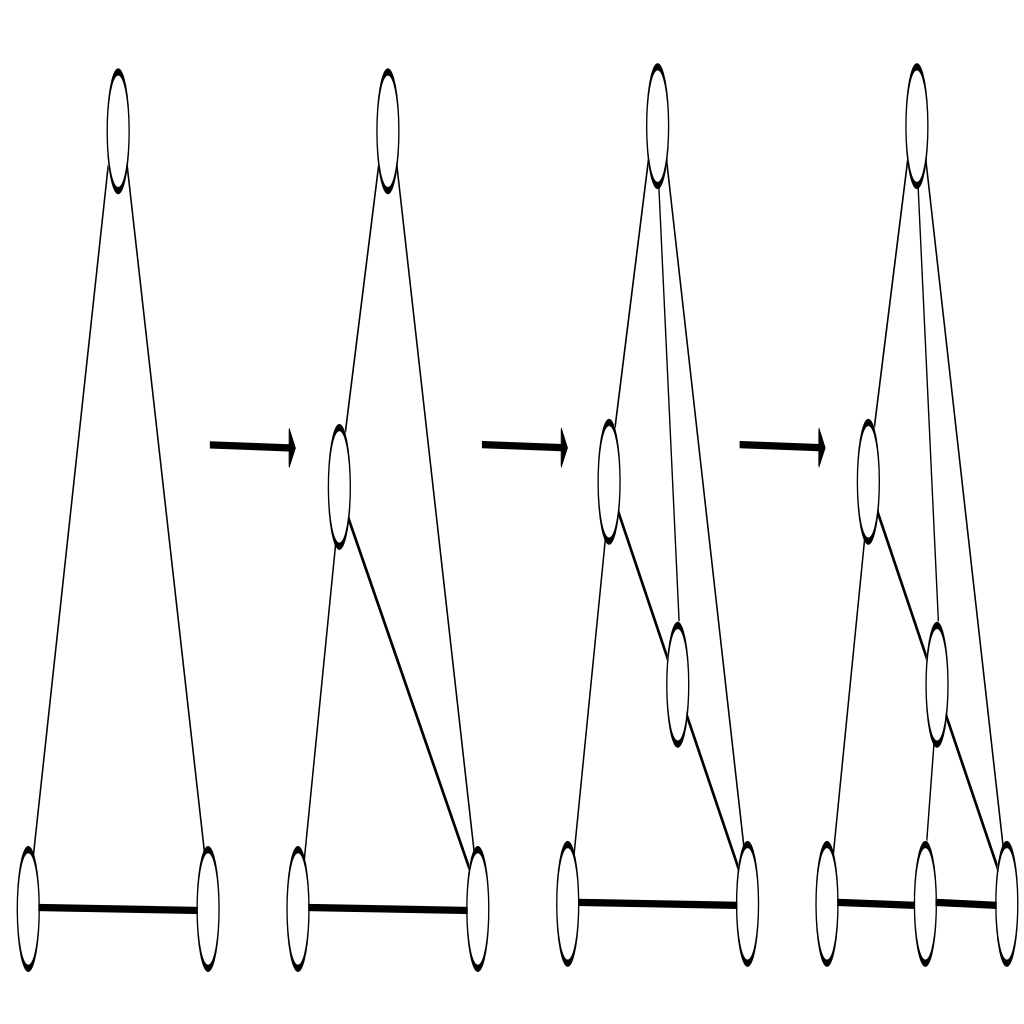
\includegraphics[width = 0.9\textwidth]{Chapter 3/3. henneberg_2.png}
    \caption{A series of constructions created solely using Henneberg Type II}
    \label{fig: henneberg 2}
\end{figure}
\noindent
By checking directly, we can verify that the graphs at each stage are indeed Laman graphs.
\end{example}

\begin{flushleft}
With the use of the rigidity matrix, or simply by observation, we can see that frameworks at each stage of the Henneberg constructions are infinitesimally rigid. 
\end{flushleft}

\begin{corollary}
\label{cor: laman => inf rigid}
Let $(G,\mathbf{p})$ be a minimally rigid framework, where $G$ is a Laman graph. Then $(G,\mathbf{p})$ is infinitesimally rigid.
\end{corollary}

\section{Rigidity vs Infinitesimal Rigidity} 

\begin{flushleft}
At this stage, we have a good understanding of what rigidity and infinitesimal rigidity are. We have seen ways to check whether a framework is infinitesimally rigid, and learned of a method to construct minimally rigid graphs. In this section, the aim is to learn how one relates with the other. 
\end{flushleft}

\begin{figure}[htbp]
    \centering
    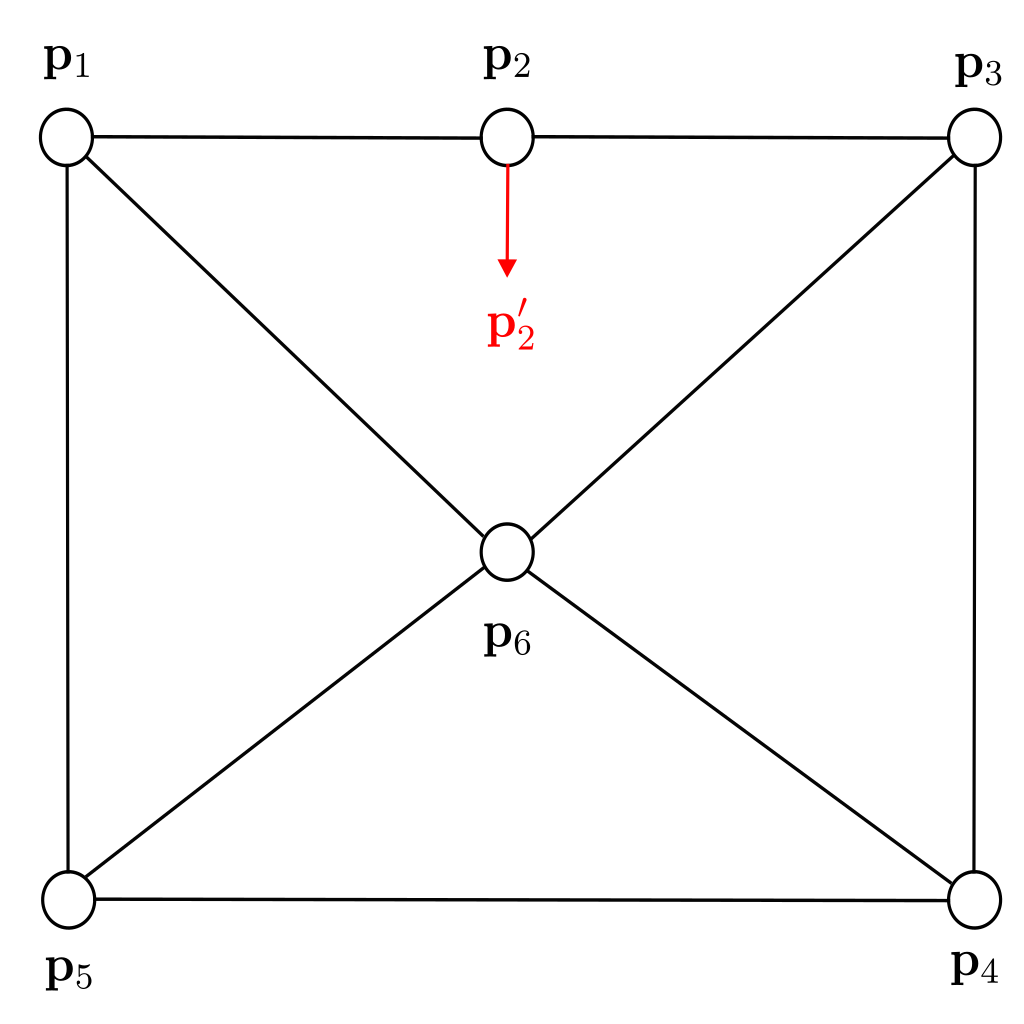
\includegraphics[width = 0.45\textwidth]{Chapter 3/6. rigid but not inf rigid.png}
    \caption{A rigid framework with an instantaneous velocity applied to $\mathbf{p}_5$ shown in red.}
    \label{fig: rigid but not inf rigid}
\end{figure}
\vspace{-4 mm}
\begin{flushleft}
To motivate this, let us consider the framework $(G,\mathbf{p})$ in Figure \ref{fig: rigid but not inf rigid}. As this framework is formed by joining two triangles together, we know it must be rigid as triangles are themselves rigid. The question is whether it is infinitesimally rigid. 
\end{flushleft}

\begin{flushleft}
Suppose we apply infinitesimal velocities of magnitude $0$ to nodes $\mathbf{p}_1$, $\mathbf{p}_2$, $\mathbf{p}_3$, $\mathbf{p}_4$, and we apply the infinitesimal velocity $\mathbf{p}'_5 \neq 0$ to node $\mathbf{p}_5$. We first verify whether these instantaneous velocities make an infinitesimal motion by checking $(\mathbf{p}_i - \mathbf{p}_j) \cdot (\mathbf{p}'_i - \mathbf{p}'_j) = 0$ for all $ij \in E(G)$. 

As each velocity vector is $0$ except for $\mathbf{p}'_5$, it follows that this is true for all the edges in $(G,\mathbf{p})$.
\end{flushleft}

\begin{flushleft}
Now, consider $(\mathbf{p}_5 - \mathbf{p}_2) \cdot (\mathbf{p}'_5 - \mathbf{p}'_2)$.The vector $(\mathbf{p}_5 - \mathbf{p}_2)$ is simply the line through the two nodes, which is non-zero, and $(\mathbf{p}'_5 - \mathbf{p}'_2) = \mathbf{p}'_5$ as $\mathbf{p}'_5$ is non-zero by assumption. As the vectors $(\mathbf{p}_5 - \mathbf{p}_2)$ and $\mathbf{p}'_5$ are not perpendicular to each other, it follows that,

\[
(\mathbf{p}_5 - \mathbf{p}_2) \cdot (\mathbf{p}'_5 - \mathbf{p}'_2) \neq 0
\]
\end{flushleft}

\begin{flushleft}
Therefore, this framework is not infinitesimally rigid. 
\end{flushleft}

\begin{flushleft}
This shows us that even though a framework might be rigid, it may not be infinitesimally rigid. Applying instantaneous velocities at a carefully selected node can very well deform a rigid structure. The converse however is true.
\end{flushleft}

\begin{theorem}
Let $(G,\mathbf{p})$ be a infinitesimally rigid framework. Then $(G,\mathbf{p})$ is rigid.
\end{theorem}

\begin{flushleft}
The proof of this theorem relies on a lot of heavy mathematics which is beyond the scope of this project, and it can be found in Asimow and Roth's paper \cite{asimow}. Therefore, infinitesimal rigidity is a stronger property than rigidity. 
\end{flushleft}

% flesh this out a little bit more. I'm unhappy with the way it ends off

\section{Circle Packings}

\begin{flushleft}
 In this last section, we finally come to circle packings and how they are defined. Additionally, we also learn how we can identify ways in which we can use the methods described earlier in order to test the rigidity of a packing. 
\end{flushleft}

\begin{figure}[htbp]
    \centering
    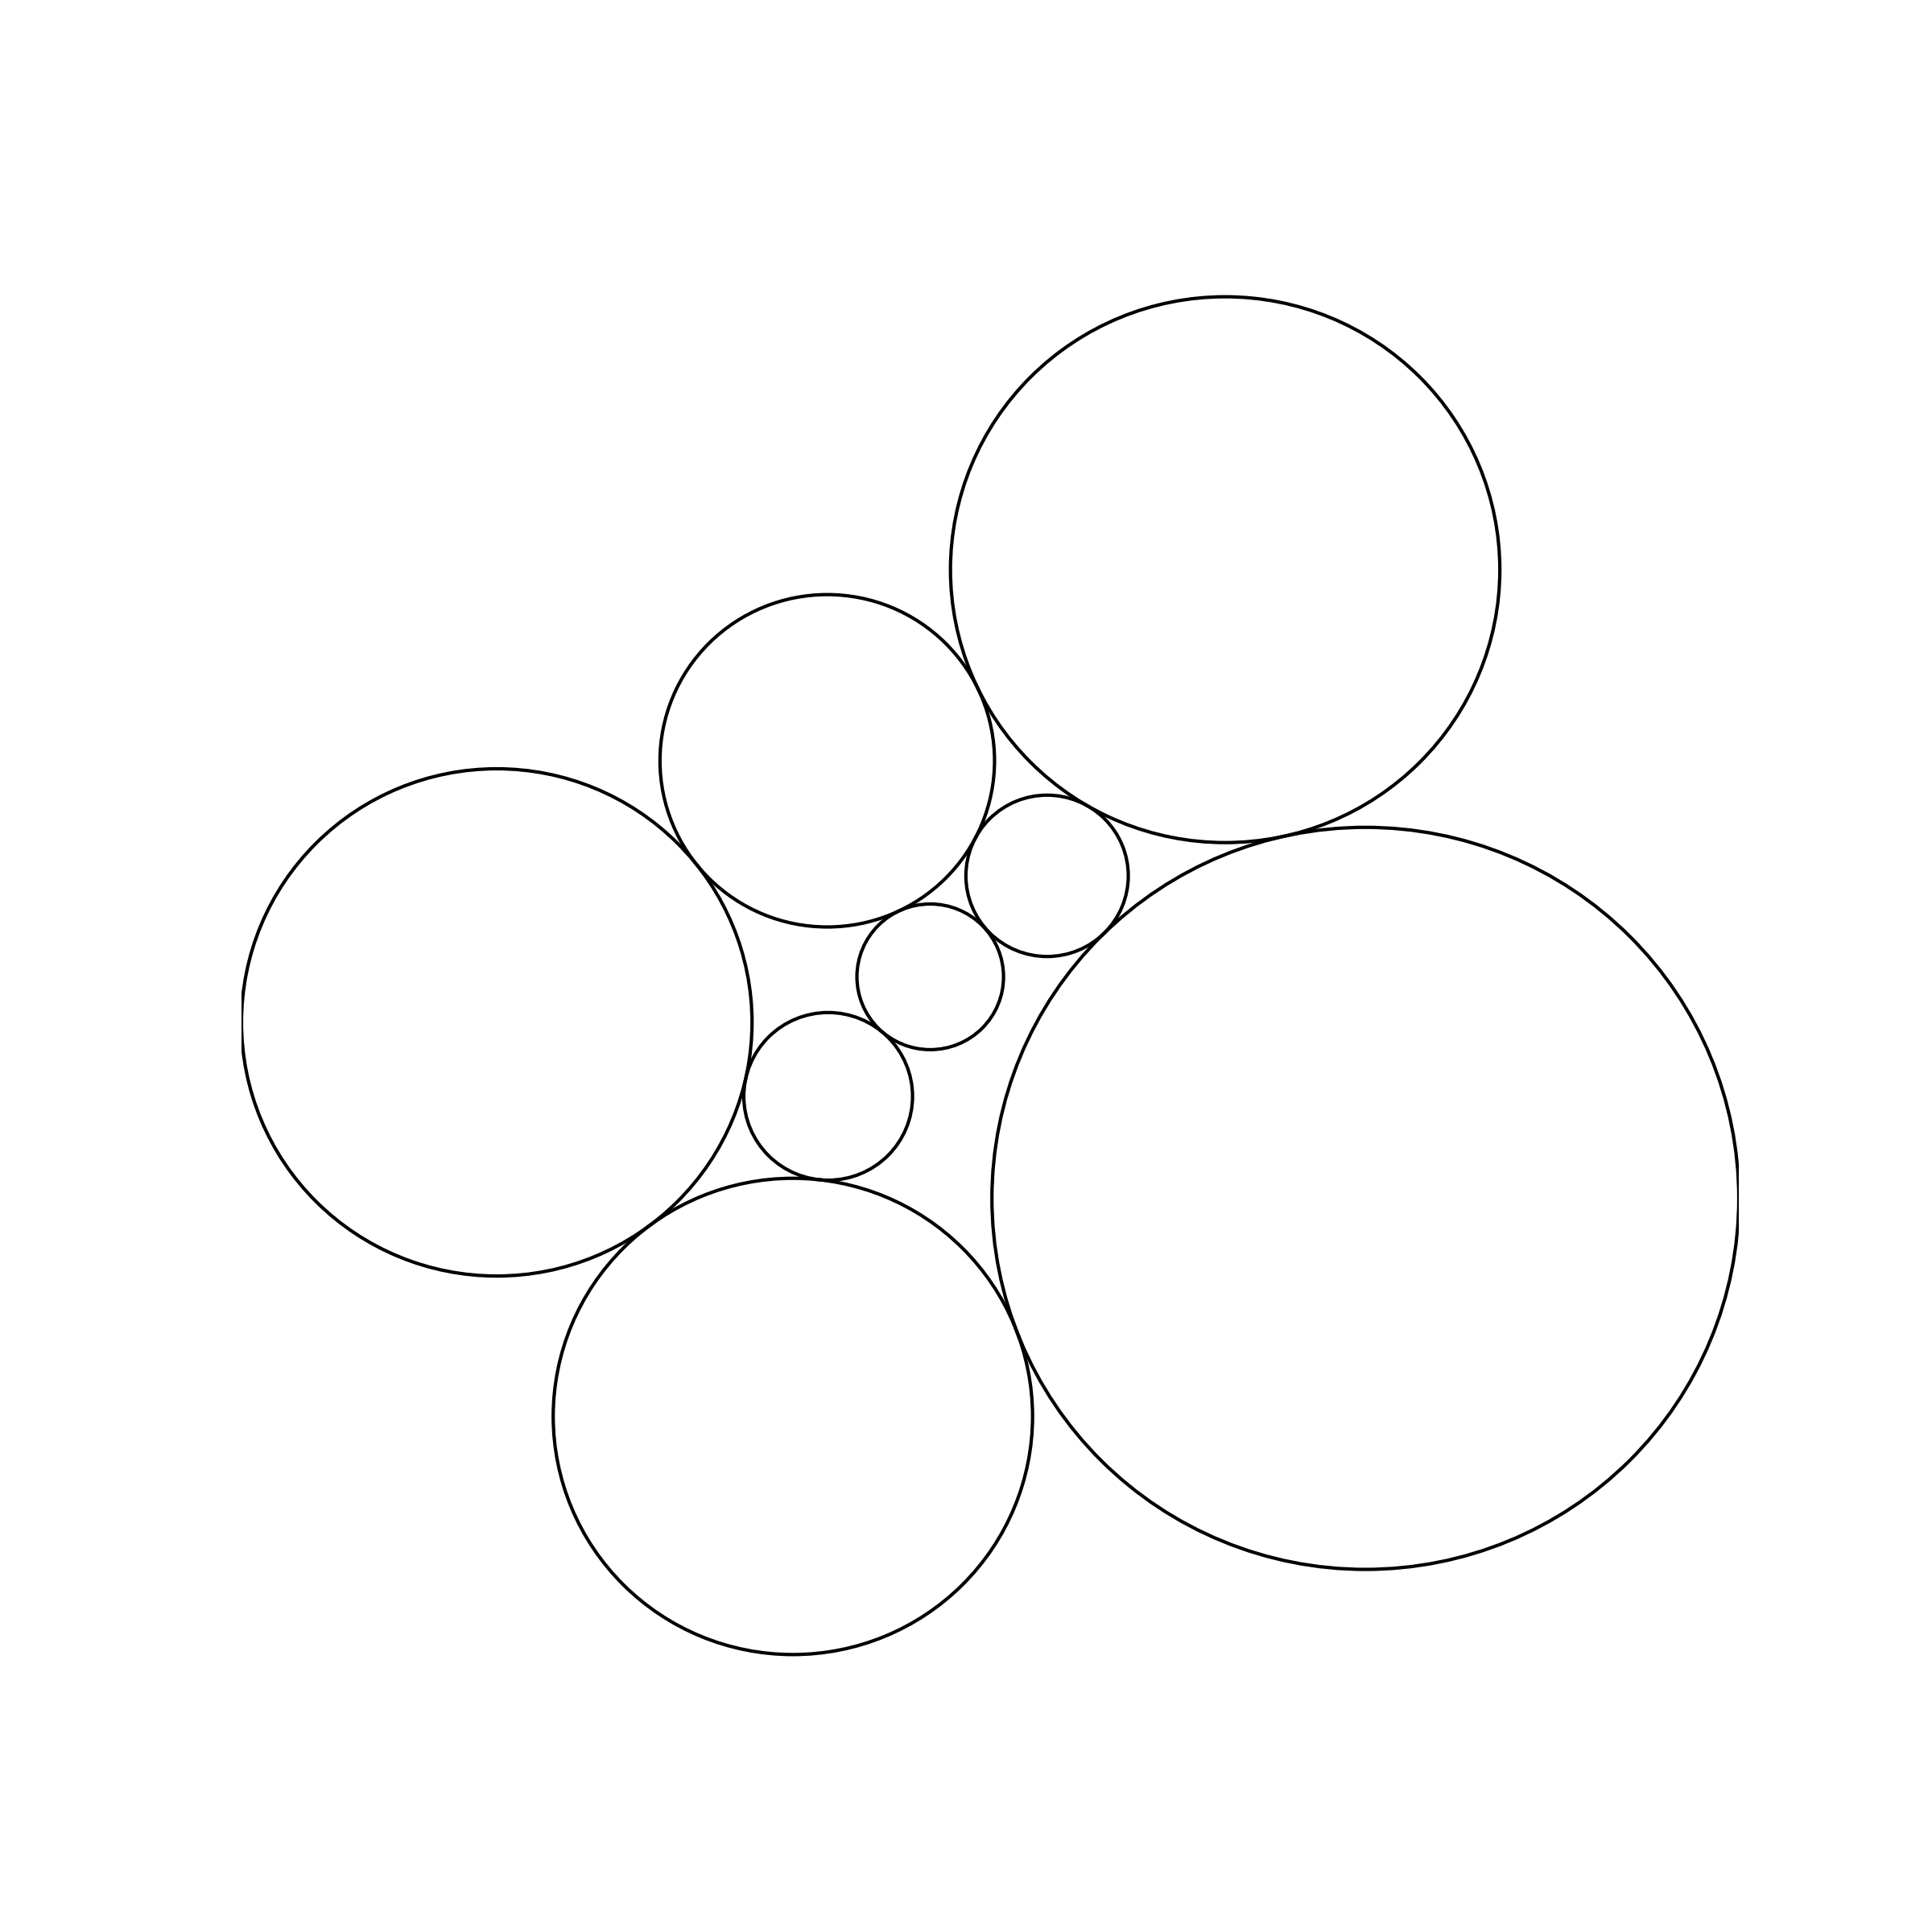
\includegraphics[width = 0.42\textwidth]{Chapter 3/7. Plain packing.png}
    \caption{A circle packing with 8 circles}
    \label{fig: circle packing example}
\end{figure}
\vspace{-4 mm}
\begin{flushleft}
Circle packings are configurations of circles satisfying preassigned patterns of tangency. They are designed such that each pair of circles may either touch tangentially, or not at all. Circles are not allowed to overlap or be contained in one another as well. An example of a circle packing is shown in Figure \ref{fig: circle packing example}. As we can see, not all of the circles have the same radius. This is necessary as the circles must be able to adjust their radii in order to fit tightly and satisfy any constraints imposed on them.
\end{flushleft}

\begin{definition}
A \textit{circle packing} is a configuration of circles $P = (C_i)$, where $i \in \mathbb{Z}^+$, in the plane $\mathbb{R}^2$ such that any
two distinct circles in P have disjoint interiors. 

\noindent
That is, distinct circles in P may be tangent, but may not overlap.
\end{definition}

\begin{flushleft}
Given a circle packing, we must now find a way to analyze its properties. Thankfully, there is a natural way to encode the qualities of a packing $P$ into a graph $G(P)$, which we call the circle packing's \textit{contact graph}.
\end{flushleft}

\begin{definition}
Let $P = (C_i)$ be a circle packing, where $i \in \mathbb{Z}^+$. Then, the \textit{contact graph} $G(P)$ of the packing $P$ is a graph where the vertex set is the set of circles in $P$, and an edge joins two vertices $u, v \in G(P)$ if an only if the circles corresponding to the vertices are tangential in $P$.
\end{definition}

\begin{flushleft}
In other words, an edge is added between two vertices in a contact graph if and only if the corresponding circles make \textit{contact}.
\end{flushleft}

\begin{flushleft}
We now have a way to encode a circle packing's properties into a graph! By observation, we can conclude that the contact graph $G(P)$ is always going to be a \hyperref[def: planar graphs]{planar} graph, as if edges were to cross over, this would imply that the corresponding circles in $P$ overlap each other. Studying a packing's contact graph allows us to invoke tools and methods we've developed so far in order to investigate the rigidity of the packing in question. 
\end{flushleft}

\begin{figure}[htbp]
    \centering
    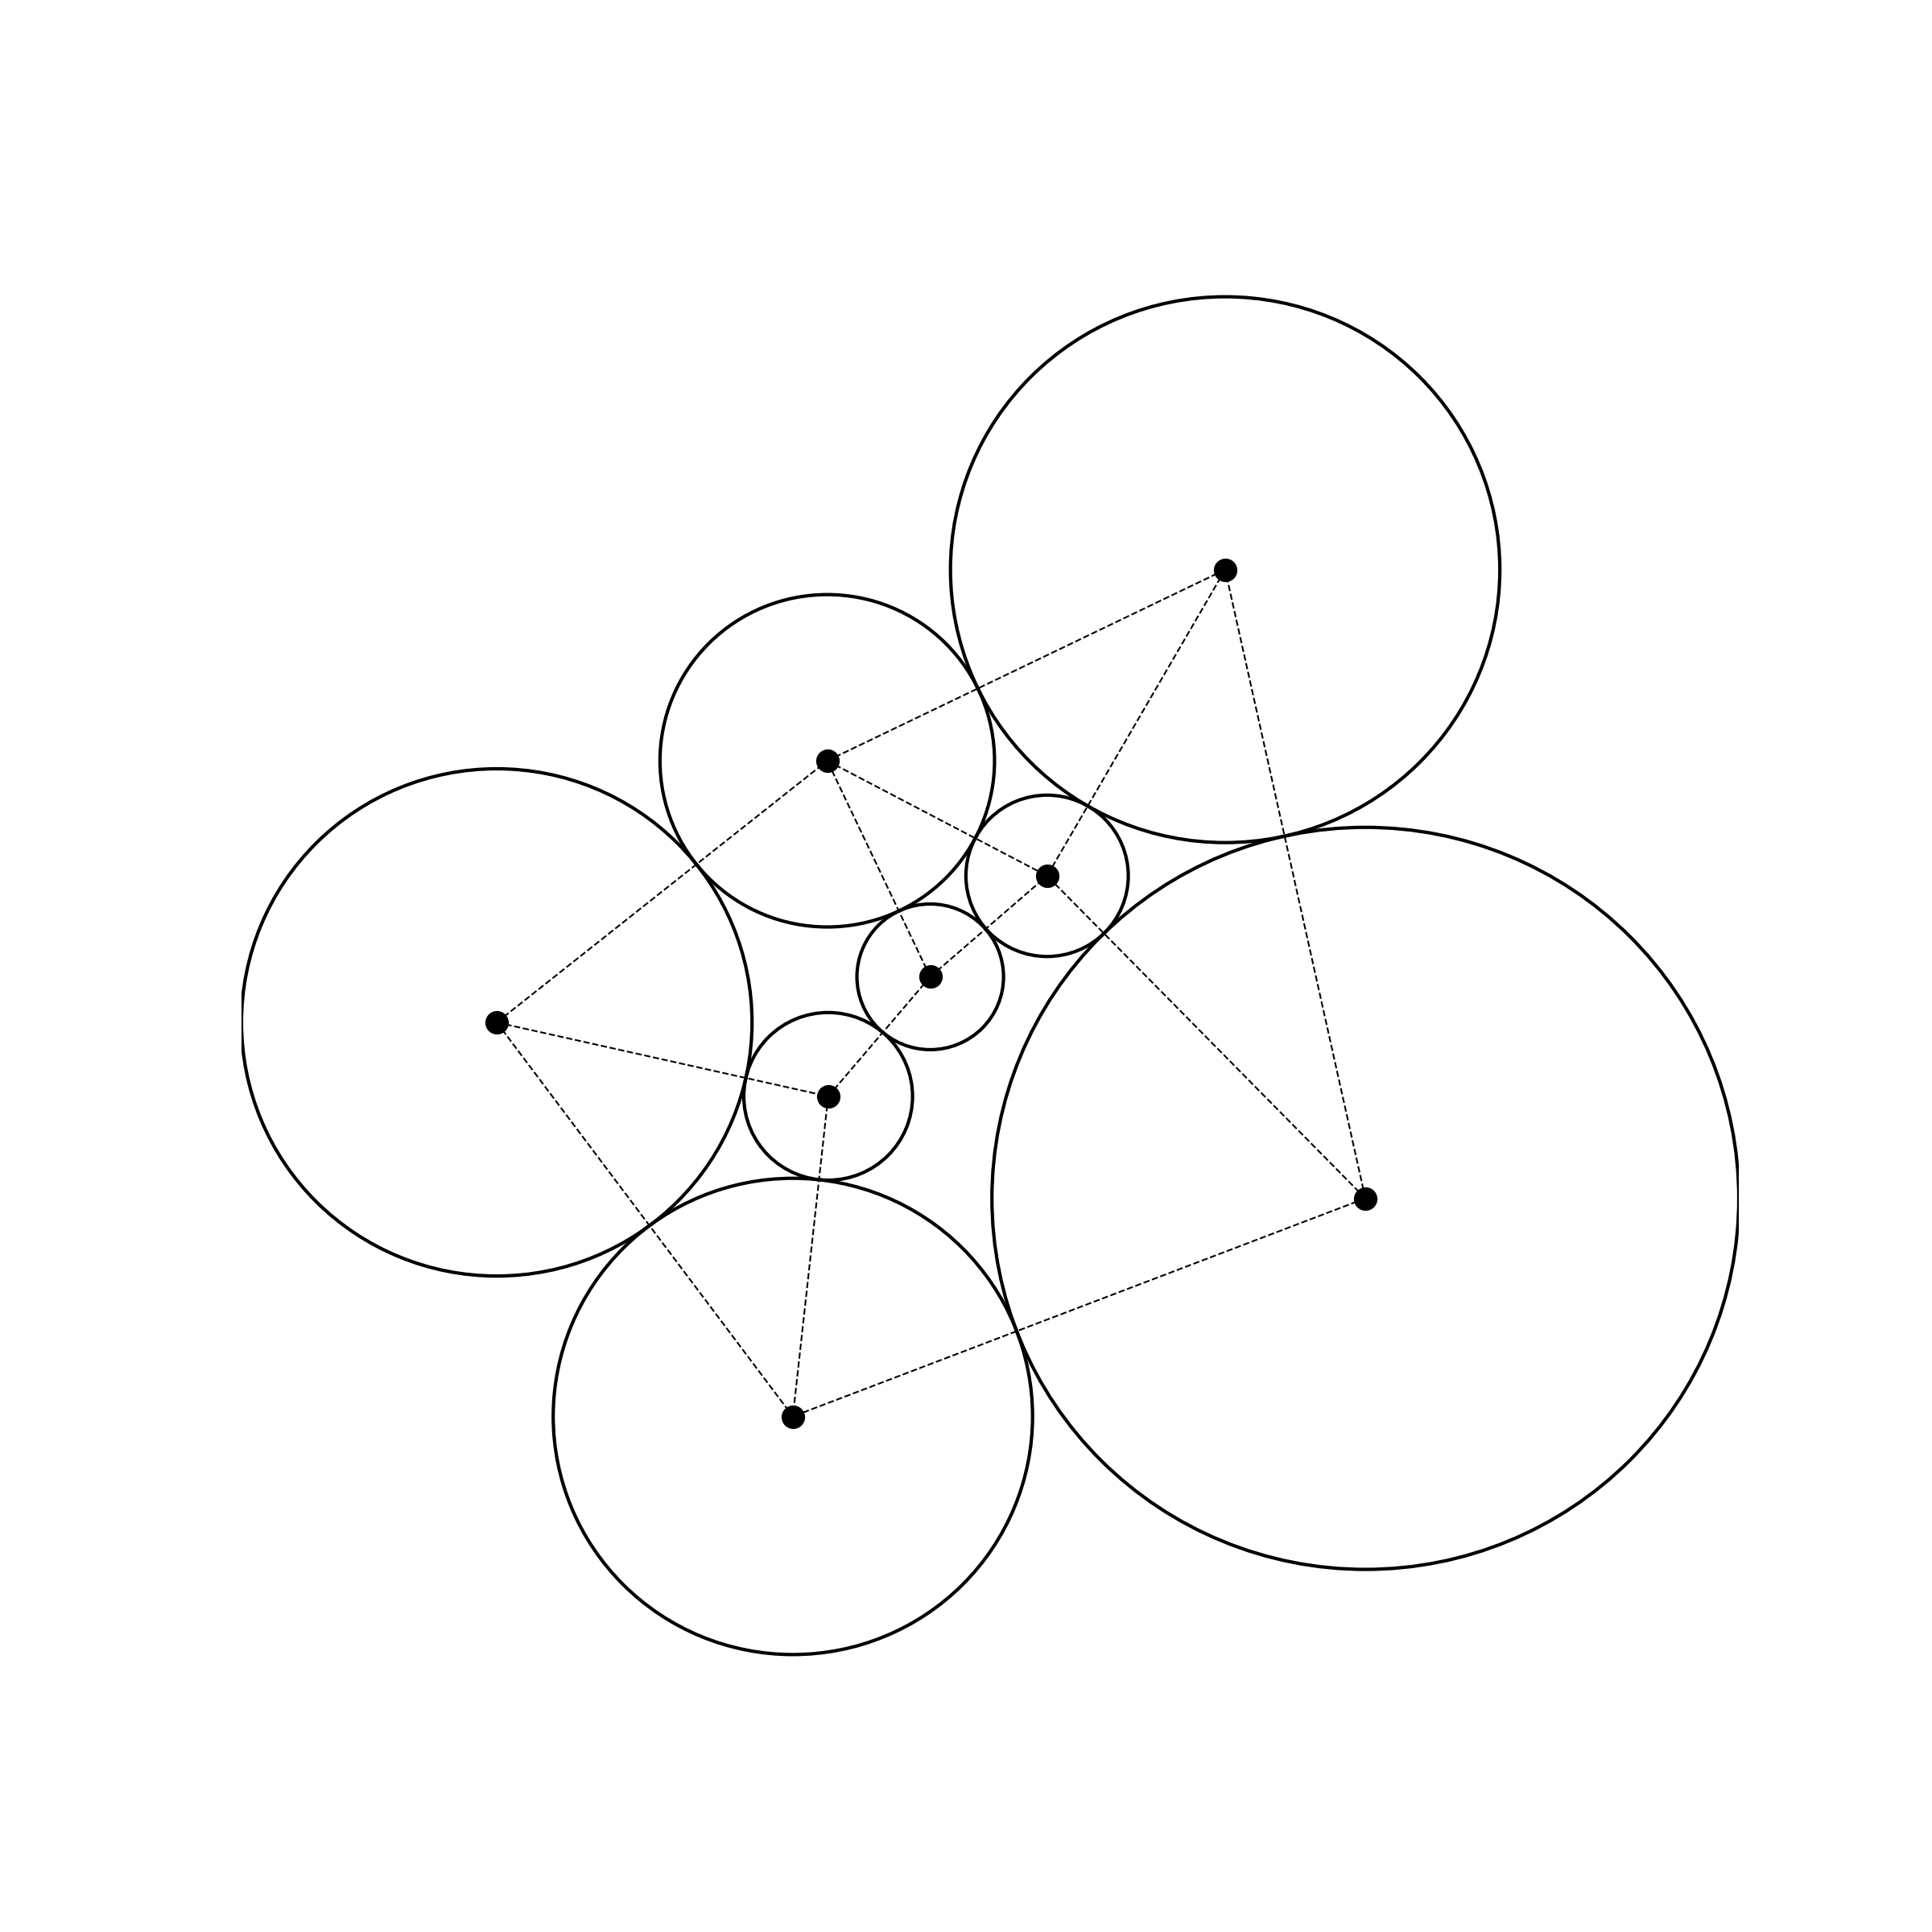
\includegraphics[width = 0.42\textwidth]{Chapter 3/8. Packing with contact.png}
    \caption{The circle packing from Figure \ref{fig: circle packing example} with its contact graph visualized}
    \label{fig: circle packing with contact}
\end{figure}
\vspace{-4 mm}
\begin{flushleft}
For a circle packing $P$, we now state that $P$ is infinitesimally rigid if its contact graph $G(P)$ is infinitesimally rigid \cite{sticky}. As rigidity does not imply infinitesimal rigidity, checking for infinitesimal rigidity is sufficient to verify the rigidity of the packing itself. 
\end{flushleft}

\begin{flushleft}
In Connelly, Gortler, and Theran's paper \cite{sticky}, the following theorem is proved.
\end{flushleft}

\begin{theorem}
Let $P = (C_i)$ be a circle packing, where $i = 1,2,\hdots, n$. Then if P has $2n-3$ contacts, it is rigid and infinitesimally rigid. If the number of contacts is fewer, then P is flexible and infinitesimally flexible.
\end{theorem}

\begin{flushleft}
This follows from investigating the contact graph $G(P)$ of a packing $P$. If the packing has $n$ circles, then there must be $n$ vertices in $G(P)$. Furthermore, if there are $2n-3$ contacts in $P$, then there must be $2n-3$ edges in $G(P)$.
\end{flushleft}

\begin{flushleft}
By Definition \ref{def: laman graph}, we know that $G(P)$ is a Laman graph, and by invoking Corollary \ref{cor: laman => inf rigid}, we deduce that $G(P)$ is infinitesimally rigid, and therefore rigid. 
\end{flushleft}

\begin{flushleft}
Finally, we need some notion of isomorphism between circle packings and graphs. Packings themselves are not unique, as there are various ways to create a circle packing originating from same graph, illustrated in Figure \ref{fig: isomorphic vs non-isomorphic packings}. To see this, we can investigate the cycles in the contact graphs of each packing. 
\end{flushleft}

\begin{flushleft}
Inspecting the graphs in Figure \ref{fig: isomorphic vs non-isomorphic packings}, we note that the original graph (a) has 3 cycles of length three. Now, comparing the contact graphs (d) and (e) to graph (a), we note that the contact graph in (d) has 3 cycles of length three, while the contact graph in (e) has only 2 cycles of length three. As the number of cycles of length three in (e) don't match those in (a), (a) and (e) must be non-isomorphic.
\end{flushleft}

\begin{flushleft}
To this end, we use a theorem that was proved by Paul Koebe in 1936, now known as the \textit{Circle Packing Theorem} \cite{circle_packing_theorem}.
\end{flushleft}

%\vspace{-3.6 mm}
\begin{theorem}
\label{thm: circle packing theorem}
Every finite planar graph $G$, where $G$ does not have multiple edges or loops between the same vertex, has a circle packing. That is, there exists a circle packing $P = (C_i)$ such that $G(P)$ is isomorphic to $G$.
\end{theorem}

\begin{flushleft}
With that, we have everything we need to set up and investigate the problem this project focuses on! By delving deep and exploring the various avenues available to us in order to check the rigidity of a given framework, we've obtained a comprehensive list of techniques at our disposal. Now, equipped with an array of theorems, we can finally get to the heart of the problem at hand!
\end{flushleft}

\begin{figure}[htbp]
    \centering
    \resizebox{0.8\textwidth}{!}{%
    \begin{tabular}{ c c } 
        \multicolumn{2}{c}{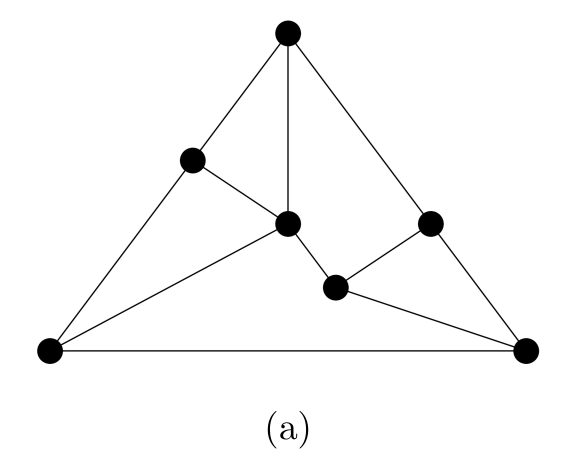
\includegraphics[width=0.3\textwidth]{Chapter 3/9. Starting graph.png}} \\ 
        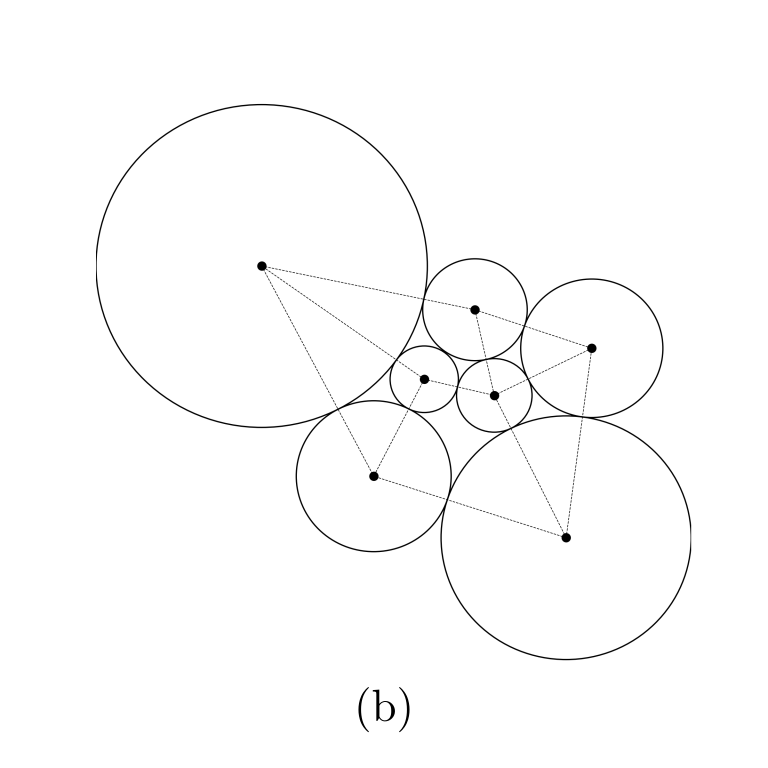
\includegraphics[width = 0.3\textwidth]{Chapter 3/10. Isomorphic packing.png} 
        & 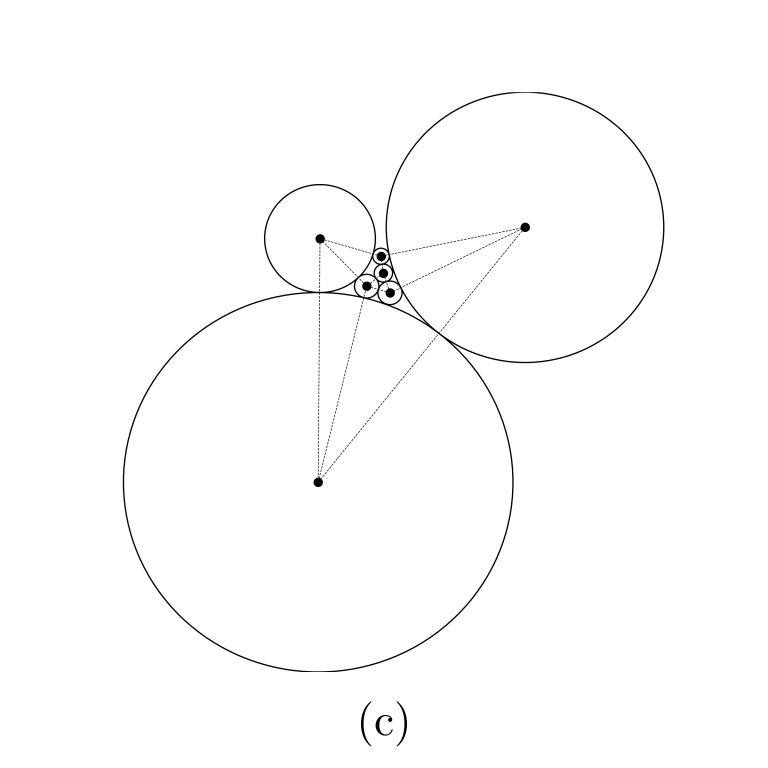
\includegraphics[width = 0.3\textwidth]{Chapter 3/11. Non-isomorphic packing.png} \\
        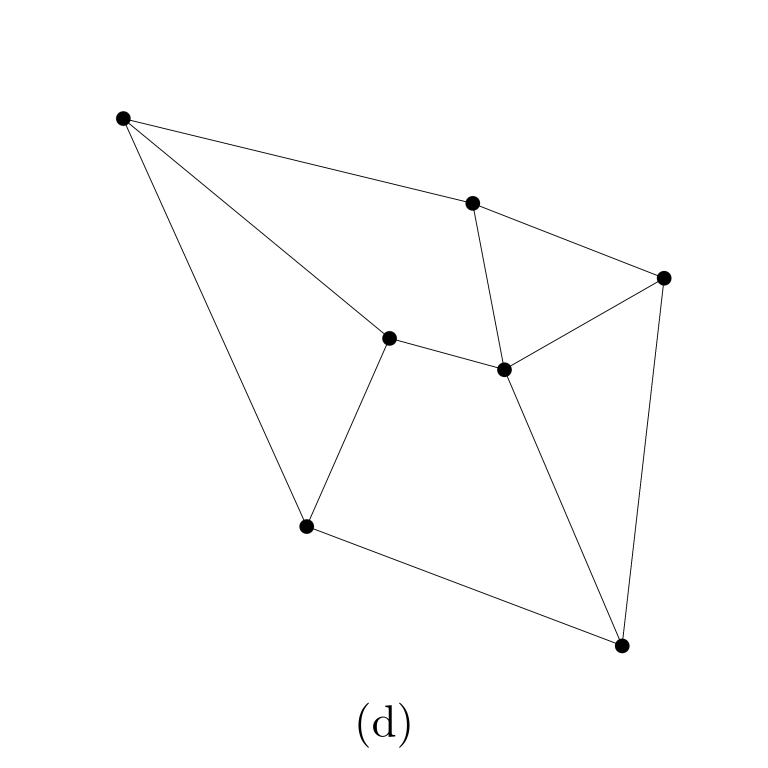
\includegraphics[width=0.3\textwidth]{Chapter 3/12. Isomorphic contact.png} &
        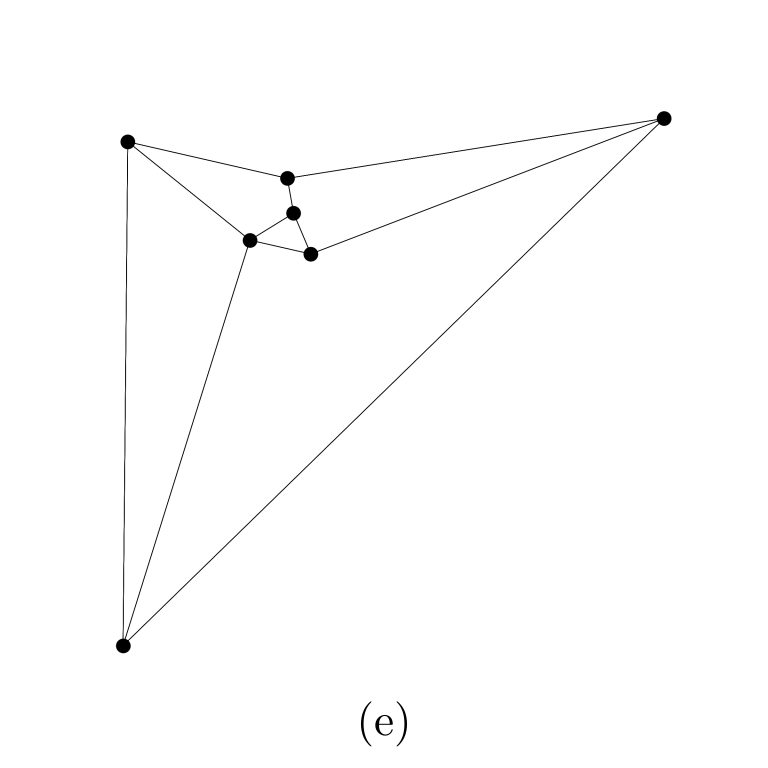
\includegraphics[width=0.3\textwidth]{Chapter 3/13. Non-isomorphic contact.png}
    \end{tabular}
    }
    \caption{A graph can have various ways in which packings can be derived from it. (a) The initial graph $G$ used to generate a circle packing. (b) A circle packing $P_1$ with a contact graph isomorphic to $G$. (c) A circle packing $P_2$ with a contact graph non-isomorphic to $G$. (d) The contact graph of $P_1$. (e) The contact graph of $P_2$.}
    \label{fig: isomorphic vs non-isomorphic packings}
\end{figure}

% lengthen the conclusion maybe?